\documentclass[11pt]{article}

\bibliographystyle{apa}
\usepackage{natbib}
\usepackage[dvips]{graphicx}
\usepackage{url}

\begin{document}

\title{When Support Vector Machines are just too slow\\(manuscript in progress)}

\author{Peter Mills\\\textit{peteymills@hotmail.com}}

\maketitle

%symbols for general kernel methods:
\newcommand{\vectorkernel}{K}
\newcommand{\scalarkernel}{K}
\newcommand{\kernelparam}{k}
\newcommand{\norm}{N}
\newcommand{\nsample}{n}
\newcommand{\dimension}{D}
\newcommand{\densityestimator}{\tilde p}
\newcommand{\bandwidth}{\sigma}
\newcommand{\coord}{x}
\newcommand{\samplecoord}{x}
\newcommand{\sample}{\vec \samplecoord}
\newcommand{\testcoord}{x}
\newcommand{\testpoint}{\vec \testcoord}
\newcommand{\point}{\vec \coord}
\newcommand{\classlabel}{y}
\newcommand{\class}{c}
\newcommand{\probability}{P}
\newcommand{\condprob}{p}
\newcommand{\kernelaverage}{W}

%symbols for SVM kernel method:
\newcommand{\svmcoeff}{w}
\newcommand{\expandedspace}{\vec\phi}
\newcommand{\svmdecision}{f}
\newcommand{\svmbordervector}{\vec v}
\newcommand{\svmborderconst}{b}

%borders classification
\newcommand{\decisionfunction}{\tilde r}
\newcommand{\diffcondprob}{r}
\newcommand{\kerneldecision}{\decisionfunction_{kern}}
\newcommand{\vbdecision}{\decisionfunction_{vb}}
\newcommand{\bordervector}{\vec b}
\newcommand{\bordernormal}{\vec v}
\newcommand{\nborder}{n_b}
\newcommand{\borderdecision}{g}
%derivative of variable bandwidth kernel estimator:
\newcommand{\distance}{d}
\newcommand{\scalarkernelderiv}{\dot \scalarkernel}

\newcommand{\svmprob}{\decisionfunction_{svm}}
\newcommand{\svmprobcoeffA}{A}
\newcommand{\svmprobcoeffB}{B}
\newcommand{\borderprob}{\decisionfunction_{border}}

%multi-classes:
\newcommand{\nclass}{n_c}
\newcommand{\multiprob}{p}


\tableofcontents

\section*{List of symbols}

%list of symbols as a latex table


\begin{tabular}{lll}
symbol & definition & first used \\ \hline
	$\lindecision$ & decision function in linear classifier & (\ref{linear_classifier})\\
	$\bordernormal$ & hyperplane normal of decision boundary & (\ref{linear_classifier})\\
	$\borderconst$ & constant value defining location of decision boundary & (\ref{linear_classifier})\\
	$\testpoint$ & test point & (\ref{linear_classifier})\\
	$\densityestimator$ & kernel density estimator & (\ref{kernel_estimator})\\
	$\vectorkernel$ & kernel function taking two vector arguments & (\ref{kernel_estimator})\\
	$\lbrace \sample_i \rbrace$ & set of training samples & (\ref{kernel_estimator})\\
	$\kernelparam$ & parameters in vector kernel & (\ref{kernel_estimator})\\
	$\norm$ & kernel normalization coefficient & (\ref{kernel_estimator})\\
	$\nsample$ & number of training samples & (\ref{kernel_estimator})\\
	$\point=\lbrace \coord_i \rbrace$ & point in the feature space & (\ref{norm_def})\\
	$\scalarkernel$ & kernel function taking a single scalar argument & (\ref{scalar_kernel_def})\\
	$\bandwidth$ & ``bandwidth'': sets the size of a scalar kernel & (\ref{scalar_kernel_def})\\
	$\probability$ & true probability density & (\ref{setting_the_bandwidth})\\
	$\dimension$ & number of dimensions in feature space & (\ref{setting_the_bandwidth})\\
	$\classlabel_i$ & class label of $i$th training sample & (\ref{kernel_classification})\\
	$\class$ & class label & (\ref{kernel_classification})\\
	$\condprob$ & conditional probability & (\ref{rdef})\\
	$\kernelsum$ & sum of the kernels at each training sample & (\ref{agf_def})\\
	$\svmcoeff$ & coefficients in weighted kernel estimator & (\ref{weighted_kernel_estimator})\\
	$\expandedspace$ & theoretical expanded feature space in kernel-based SVM & (\ref{phi_def})\\
	$\svmdecision$ & raw decision function in binary SVM & (\ref{decision_function0})\\
	$\svmcost$ & cost parameter in SVM for reducing over-fitting & (\ref{svmcost}) \\
	$\diffcondprob$ & difference in conditional probabilities & (\ref{rdef}) \\
	$\decisionfunction$ & decision function which is estimator of $\diffcondprob$ & (\ref{rdef})\\
	$\kerneldecision$ & kernel estimator for $\diffcondprob$ & (\ref{kernel_decision}) \\
	$\vbdecision$ & variablekernel estimator for $\diffcondprob$ & (\ref{vb_kernel_r}) \\
	$\lbrace \bordervector_i \rbrace$ & set of vectors defining the class border & (\ref{border_decision}) \\
	$\lbrace \bordernormal_i \rbrace$ & set of normals to the class border & (\ref{border_decision}) \\
	$\nborder$ & number of border vectors & (\ref{border_decision}) \\
	$\borderdecision$ & raw decision function for border classification & (\ref{border_decision}) \\
	$\distance$ & distance in feature space & (\ref{kernel_gradient}) \\
	$\scalarkernelderiv$ & derivative of a scalar kernel, $\scalarkernel$ & (\ref{kernel_gradient}) \\
	$\svmprob$ & LIBSVM estimator for $\diffcondprob$ & (\ref{svm_prob}) \\
	$\svmprobcoeffA$ & coefficient used in $\svmprob$ & (\ref{svm_prob}) \\
	$\svmprobcoeffB$ & coefficient used in $\svmprob$ & (\ref{svm_prob}) \\
	$\borderprob$ & borders estimator for $\diffcondprob$ & (\ref{border_probability}) \\
	$\lmult$ & Lagrange multiplier in multi-class problem & (\ref{multiclass}) \\
	$\rbkernelparam$ & parameter used for Gaussian kernels in SVM & S \ref{results_section} \\
	$\lbrace \confusion_{ij} \rbrace$ & confusion matrix & (\ref{accuracy}) \\
	$\ntest$ & number of test points & (\ref{accuracy}) \\
	$\priorentropy$ & entropy of the prior distribution & (\ref{prior_entropy}) \\
	$\posteriorentropy$ & entropy of the posterior distribution & (\ref{posterior_entropy}) \\
	$\UC$ & uncertainty coefficient (normalized channel capacity) & (\ref{uncertainty_coefficient})
\end{tabular}





\section{Introduction}

\section{Theory}

\subsection{Kernel estimation}

A kernel is a scalar function of two vectors. Kernel functions are used for 
non-parametric density estimation. A typical ``kernel-density estimator"
looks like this:
\begin{equation}
	\densityestimator(\testpoint) = \frac {1}{\norm \nsample} \sum_{i=1}^\nsample \vectorkernel(\sample_i, \testpoint, \kernelparam)
\end{equation}
where $\densityestimator$ is an estimator for the density, $\probability$, 
$\vectorkernel$ is the kernel function,
$\lbrace \sample_i \rbrace$ are a set of samples, 
$\nsample$ is the number of samples,
$\testpoint$ is the test point,
and $\kernelparam$ is a set of parameters. 
The normalization coefficient, $\norm$, normalizes $\vectorkernel$:
\begin{equation}
	\norm = \int_V \vectorkernel(\point, \point^\prime, \kernelparam) \mathrm d \point^\prime
\end{equation}

The method can be used for statistical classification by simply comparing
results from the different classes:
\begin{equation}
	\class = \arg \min_i \sum_{j|\classlabel_j = i} K(\sample_j, \testpoint, \kernelparam)
\end{equation}
where $\classlabel_j$ is the class of the $j$th sample. Naturally the method can also
be used to estimate both the joint and conditional probabilities 
($\condprob(\class, \vec x)$ and $\condprob(\class |\vec x)$ respectively). 
More on this later.

If the same kernel is used for every sample and every test point, the estimator
may be sub-optimal, particularly in regions of very high or very low density.
\citep{Terrell_Scott1992, Mills2011}.
There are at least two solutions to this problem.
In a ``variable-bandwidth'' estimator, the coefficients, $\kernelparam$, depend in some
way on the density. Since the density itself is normally unavailable, the
estimated density is used as a proxy. In \citet{Terrell_Scott1992} and
\citet{Mills2011} 
Let the kernel function takes the following form:
\begin{equation}
	\vectorkernel(\point, \point^\prime, \bandwidth) = \scalarkernel \left (\frac{|\point - \point^\prime|}{\bandwidth} \right )
\end{equation}
where $\bandwidth$ is the ``bandwidth''. 
In \citet{Mills2011}, $\bandwidth$ is made proportional to the density:
\begin{equation}
	\bandwidth \propto \frac{1}{\probability^{1/\dimension}} \approx \frac{1}{\densityestimator^{1/\dimension}}
\end{equation}
where $\dimension$ is the dimension of the feature space.
Since the normalization coefficient, $\norm$, must include the factor,
${\bandwidth^\dimension}$, some rearrangement shows that:
\begin{equation}
	\frac{1}{\nsample} \sum_i \scalarkernel \left (\frac{|\testpoint - \sample_i|}{\bandwidth} \right ) = \kernelaverage = const.
\end{equation}
This is a generalization of the $k$-nearest-neighbours scheme in which the
free parameter, $\kernelaverage$, takes the place of $k$. \citep{Mills2009, Mills2011}
The bandwidth, $h$, can be solved
for using any numerical, one-dimensional root-finding algorithm.
The bandwidth is determined at each test point.

Another method of improving the performance of a kernel-density estimator
is to add a series of variable coefficients:
\begin{equation}
	\densityestimator(\testpoint) = \sum_i \svmcoeff_i \vectorkernel(\sample_i, \testpoint, \kernelparam)
\end{equation}
The coefficients, $\lbrace \svmcoeff_i \rbrace$, are found through an optimization
procedure designed to minimize the error [citation...]. In the most popular
form of this kernel method, Support Vector Machines (SVM), the coefficients
are the result of a complex, dual optimization procedure which minimizes
the classification error. We will briefly outline this procedure.

\subsection{Support Vector Machines}

The basic ``trick'' of kernel-base SVM methods is to replace a dot product
with the kernel function in the assumption that it can be rewritten
as a dot product of a transformed and expanded feature space:
\begin{equation}
	\vectorkernel(\point, \point^\prime) = \expandedspace(\point) \cdot \expandedspace(\point^\prime)
\end{equation}
For simplicity we have ommitted the kernel parameters.
$\expandedspace$ is a vector function of the feature space.
The simplest example of a kernel function that has a closed, analytical and
finite-dimensional $\expandedspace$ is the square of the dot product:
\begin{eqnarray}
	\vectorkernel(\point, \point^\prime) & = & (\point \cdot \point^\prime)^2 \\ \nonumber
					 & = & (\coord_1^2, \coord_2^2, \coord_3^2, ..., \sqrt{2} \coord_1 \coord_2, \sqrt{2} \coord_1 \coord_3, ... \sqrt{2} \coord_2 \coord_3, ...) \cdot \\ \nonumber
      & &	 ({\coord^\prime_1}^2, {\coord^\prime}_2^2, {\coord^\prime}_3^2, ..., \sqrt{2} \coord^\prime_1 \coord^\prime_2, \sqrt{2} \coord^\prime_1 \coord^\prime_3, ... \sqrt{2} \coord^\prime_2 \coord^\prime_3, ...) 
\end{eqnarray}
but it should be noted that in more complex cases, 
there is no need to construct $\expandedspace$ since it is replaced by the 
kernel function, $\vectorkernel$, in the final analysis.

In a binary SVM classifier, the classes are separated by a single hyper-plane
defined by $\svmbordervector$ and $\svmborderconst$.
In a kernel-based SVM, this hyperplane bisects not the regular feature
space, but the theoretical, transformed space defined by the function,
$\expandedspace(\point)$.
The {\it decision value} is calculated via a dot product:
\begin{equation}
	\svmdecision(\testpoint)=\svmbordervector \cdot \expandedspace(\testpoint) + \svmborderconst
	\label{decision_function0}
\end{equation}
and the class determined by the sign of the decision value:
\begin{equation}
	\class=\frac{\svmdecision}{|\svmdecision|}
	\label{class_value}
\end{equation}
where for convenience, the class labels are given by $c \in \lbrace -1, 1 \rbrace$.

In the first step of the minimization procedure, 
the magnitude of the border normal, $\svmbordervector$, 
is minimized subject to the constraint that there are no classification 
errors:
\begin{eqnarray}
	\min_{\svmbordervector, \svmborderconst} \frac{1}{2} | \svmbordervector | \\ \nonumber
	\svmdecision(\sample_i) \classlabel_i \ge 1
\end{eqnarray}
Introducing the coefficients, $\lbrace \svmcoeff_i \rbrace$, 
as Lagrange multipliers on the constraints:
\begin{equation}
	\min_{\svmbordervector, b} \left \lbrace \frac{1}{2} | \svmbordervector | - \sum_i \svmcoeff_i \left [ \svmdecision(\sample_i) \classlabel_i -1 \right ] \right \rbrace
\end{equation}
generates the following pair of analytic expressions:
\begin{eqnarray}
	\sum_i \svmcoeff_i \classlabel_i & = & 0 \\
	\svmbordervector & = & \sum_i \svmcoeff_i \classlabel \expandedspace(\sample_i) \label{border_vector_equation}
\end{eqnarray}
through setting the derivatives w.r.t. the minimizers to zero.
Substituting the second equation, (\ref{border_vector_equation}),
into the decision function in (\ref{decision_function0}) produces the following:
\begin{equation}
	\svmdecision(\testpoint) = \sum_i \svmcoeff_i \classlabel_i \vectorkernel (\testpoint, \sample_i) + \svmborderconst
	\label{svm_decision}
\end{equation}
Meanwhile, the final, dual, quadratic optimization problem looks like this:
\begin{eqnarray}
	\max_{\lbrace \svmcoeff_i \rbrace} & \sum_i \svmcoeff_i 
	- \frac{1}{2} \sum_{i, j} \svmcoeff_i \svmcoeff_j \classlabel_i \classlabel_j \vectorkernel(\sample_i, \sample_j) \label{dual_problem} \\
	& \svmcoeff_i \ge 0 \label{constraint1} \\
	& \sum_i \svmcoeff \classlabel_i = 0 \label{constraint2}
\end{eqnarray}
There are a number of refinements that can be applied to the optimization
problem in (\ref{dual_problem})-(\ref{constraint2}), chiefly to reduce over-fitting and to add
some ``margin'' to the decision border to allow for the possibility of
classification errors.
For instance, substitute the following for (\ref{constraint1}):
\begin{equation}
 0 \le \svmcoeff_i \le C
\end{equation}
where $C$ is the cost \citep{kernel_intro}.
Mainly we are concerned here with the decision
function in (\ref{svm_decision}) since the initial fitting will be done with
an external software package, namely LIBSVM \citep{Chang_Lin2011}.

Two things should be noted. First, the function $\expandedspace$ appears in
neither the final decision function, (\ref{svm_decision}), nor in the
optimization problem, (\ref{dual_problem}). Second, while the use of
$\expandedspace$ implies that the time complexity of the decision function 
could be $O(1)$ as in a parametric statistical model, in actual fact it is
dependent on the number of non-zero values in $\lbrace \svmcoeff_i \rbrace$.
While the coefficient set, $\lbrace \svmcoeff_i \rbrace$, does tend to be sparse,
nonetheless in most real problems the number of non-zero coefficients is
proportional to the number of samples, $\nsample$, producing a time complexity
of $O(\nsample)$. Thus for large problems, calculating the decision value will
be slow, just as in other kernel estimation problems.

The advantage of SVM lies chiefly in its accuracy since it is minimizing the
classification error whereas a more basic kernel method is more ad hoc
and does little more than sum the number of samples weighted by distance.

\subsection{Border classification}

\label{border_method}

In kernel SVM, the decision border exists only implicitly in a hypothetical,
abstract space. Even in linear SVM, if the software is generalized to 
recognize the simple dot product as only one among many possible kernels,
then the decision function may be built up, as in (\ref{svm_decision})
through a sum of weighted kernels. This is the case for LIBSVM.
The advantage of an explicit decision border as in (\ref{decision_function0})
is that it is fast. The problem with a linear border is that, except for a
small class of problems, it is not very accurate.

In the binary classification method described in \citet{Mills2011},
a non-linear decision border is built up piece-wise from a collection of linear borders.
It is essentially a root-finding procedure for a decision function,
such as $\svmdecision$ in (\ref{svm_decision}).
Let $\decisionfunction$ be a decision function. In the ideal case, it should
be an accurate estimator for the difference in conditional probabilities:
\begin{equation}
	\decisionfunction(\point) = \diffcondprob(\point) = 
	\condprob(1|\point) - \condprob(-1|\point)
\end{equation}
where $\condprob(\class|\point)$ represents the conditional probabilities of
a binary classifier having labels $\class \in \lbrace -1, 1 \rbrace$.
For a simple kernel estimator, for instance, 
$\diffcondprob$ is estimated as follows:
\begin{equation}
	\kerneldecision(\testpoint) = \frac{\sum_i \classlabel_i \vectorkernel(\testpoint, \sample_i)}{\sum_i \vectorkernel(\testpoint, \sample_i)}
	\label{kernel_decision}
\end{equation}
where $\classlabel_i \in \lbrace -1, 1 \rbrace$.
For a variable bandwidth kernel estimator, this works out to:
\begin{equation}
	\vbdecision(\testpoint) = \frac{1}{\kernelaverage} \sum_i \classlabel_i \scalarkernel \left (\frac{|\testpoint - \sample_i|}{\bandwidth(\testpoint)} \right )
	\label{vb_kernel_r}
\end{equation}
A variable bandwidth kernel-density estimator with a Gaussian kernel,
$\scalarkernel(x)=\exp(-x^2/2)$ we will refer to as an ``Adaptive Gaussian
Filter'' or AGF for short.

The procedure is as follows: pick a pair of points on either side of the decision
boundary (the decision function has opposite signs). Good candidates are one
random training sample from each class. Then, zero the decision function
along the line between the points. This can be done as many times as needed
to build up a good representation of the decision boundary.
We now have a set of points, $\lbrace \bordervector_i \rbrace$, such that
$\decisionfunction(\bordervector_i)=0$ for every $i=[1..\nborder]$ where
$\nborder$ is the number of border samples.

Along with the border samples,  $\lbrace \bordervector_i \rbrace$, we also
collect a series of normal vectors, $\lbrace \bordernormal_i \rbrace$
such that:
\begin{equation}
\bordernormal_i=\nabla_{\point}{\decisionfunction |_{\point=\bordervector_i}}
\end{equation}
With this system, determining the class is a two step proces.
First, the nearest border to the test point is found.
Second, we define a new decision function, $\borderdecision$, 
similar to (\ref{decision_function0}), through a dot product with the normal:
\begin{eqnarray}
	i & = & \arg \min_j |\testpoint - \bordervector_j| \\ \nonumber
	\borderdecision(\testpoint) & = & \bordernormal_i \cdot (\testpoint - \bordervector_i)
	\label{border_decision}
\end{eqnarray}
The class is determined by the sign of the decision function as in 
(\ref{class_value}).
The time complexity is completely independent of the number
of training samples, rather it is linearly proportional to the number of
border vectors, $\nborder$, a tunable parameter. The number required for
accurate classifications is dependent on the complexity of the decision
border.

The gradient of the variable-bandwidth kernel estimator in 
(\ref{vb_kernel_r}) is:
\begin{equation}
	\frac{\partial \vbdecision}{\partial \testcoord_j} = 
	\frac{2 \bandwidth}{\kernelaverage} \sum_i \classlabel_i
	\scalarkernelderiv \left (\frac{\distance_i}{\bandwidth} \right )
	\left [\frac{\testcoord_j - \samplecoord_{ij}}{\distance_i} 
	- \distance_i \frac{\sum_k \scalarkernelderiv \left (\frac{\distance_k}{\bandwidth} \right )
	\frac{\testcoord_j - \samplecoord_{kj}}{\distance_k}}
{\sum_k \distance_k \scalarkernelderiv \left (\frac{\distance_k}{\bandwidth} \right )} \right ]
\end{equation}
where $\distance_i=|\point - \sample_i|$ is the distance between the 
test point and the $i$th sample and $\scalarkernelderiv$ is the derivative
of $\scalarkernel$.
For AGF, this works out to:
\begin{equation}
	\frac{\partial \vbdecision}{\partial \testcoord_j} = 
	\frac{1}{\bandwidth^2 \kernelaverage} \sum_i \classlabel_i
	\scalarkernel \left (\frac{\distance_i}{\bandwidth} \right )
	\left [\samplecoord_{ij} - \testcoord
	- \distance_i^2 \frac{\sum_k \scalarkernel \left (\frac{\distance_k}{\bandwidth} \right )
	\left (\samplecoord_{kj} - \testcoord \right )}
{\sum_k \scalarkernel \left (\frac{\distance_k}{\bandwidth} \right )\frac{1}{\distance_k^2}} \right ]
\end{equation}
where $K(x)=\exp(-x^2/2)$ \citep{Mills2011}.

In LIBSVM, conditional probabilities are estimated by applying a
sigmoid function to
the raw SVM decision function, $\svmdecision$, in (\ref{svm_decision}):
\begin{equation}
	\svmprob(\testpoint) = \tanh \left (\frac{\svmprobcoeffA \svmdecision(\testpoint)+ \svmprobcoeffB}{2} \right )
	\label{svm_prob}
\end{equation}
where $\svmprobcoeffA$ and $\svmprobcoeffB$ are coefficients derived from
the training data via
nonlinear least-squares fitting \citep{Lin_etal2007, Chang_Lin2011}.

The gradient of the revised SVM decision function, above, is:
\begin{equation}
	\nabla_{\point} {\svmprob} = \left [1 - \svmprob^2(\point) \right ] \sum_i \svmcoeff_i \classlabel_i \nabla_{\point} \vectorkernel(\point, \sample_i)
\end{equation}

Gradients of the initial decision function are useful not just to derive normals to
the decision boundary, but also as an aid to root finding when searching for
border samples. If the decision function used to compute the border samples
represents an estimator for the
difference in conditional probabilities, then the raw decision value,
$\borderdecision$,
derived from the border sampling technique in (\ref{border_decision})
can also return estimates of the conditional probabilities with little
extra effort and little loss of accuracy--also using a sigmoid function:
\begin{equation}
	\borderprob(\testpoint) = \tanh \left [\borderdecision (\testpoint) \right ]
	\label{border_probability}
\end{equation}
This assumes that the class posterior probabilities,
$\condprob(\point | c)$, are approximately Gaussian near the border
\citep{Mills2011}.

The border classification algorithm, returns an estimator,
$\borderprob$, for the difference in conditional probabilities of
a binary classifier using
equations (\ref{border_decision}) and (\ref{border_probability}).
It can be trained with the functions $\kerneldecision$ in (\ref{kernel_decision}),
$\vbdecision$ in (\ref{vb_kernel_r}), $\svmprob$ in (\ref{svm_prob}),
or any other 
continuous, differentiable, non-parametric estimator for the difference
in conditional probabilities, $\diffcondprob$.
At the cost of a small reduction in accuracy,
it has the potential to drastically reduce classification time for kernel
estimators and other non-parametric statistical classifiers,
especially for large training datasets,
since it has $O(\nborder)$ time complexity instead of $O(\nsample)$
complexity, where $\nborder$, the number of border samples, is a free parameter.
The actual number chosen
can trade off between speed and accuracy with rapidly diminishing returns
beyond a certain point. 
One hundred border samples ($\nborder=100$) is usually sufficient.
The computation of $\borderprob$ also involves very simple operations--
floating point addition, multiplication and numerical comparison, with no
transcendental functions except for the very last step (which can be omitted)--so the coefficient for the time complexity will be small.

A border classifier trained with AGF will be referred to as an ``AGF-borders''
classifier while a border classifier trained with SVM estimates will
be referred to as an ``SVM-borders'' classifier.

\subsection{Multi-class classification}

The border classification algorithm, like SVM, only works for binary 
classification problems. It is quite easy to generalize a binary classifier
to perform multi-class classifications by using several of them and the
number of ways of doing so grows exponentially with the number of classes.
Since LIBSVM uses the ``one-versus-the-rest'' method \citep{Hsu_Lin2002} of 
multi-class classification, this is the one we will adopt. 

A major advantage of the
borders classifier is that it returns probability estimates.
These estimates are based on a simple interpolation, however, so they may
not always be accurate and we are interested in comparing their accuracy
with that of the original estimates. Therefore, the multi-class method
should also solve for the conditional probabilities in addition to returning
the class label.

In a one-vs.-the rest scheme, the multi-class conditional probabilities 
can be related to those of the binary classifiers as follows:
\begin{equation}
	\diffcondprob_{ij}(\point) = \frac{\condprob(j|\point) - \condprob(i|\point)}{\condprob(i|\point) + \condprob(j|\point)}
\end{equation}
where $i=[1..\nclass-1]$, $\nclass$ is the number of classes, $j>i$,
and $\diffcondprob_{ij}$ is the difference in conditional probabilities of
the binary classifier that discriminates between the $i$th and $j$th classes.
\citet{Wu_etal2004} transform this problem into the following linear system:
\begin{eqnarray}
	\sum_i \frac{1}{4} \left [ \multiprob_i \sum_{j|j \ne i} (\decisionfunction_{ij} + 1)^2 - \multiprob_i (\decisionfunction_{ij}^2 - \decisionfunction_{ij} - 2) \right ] + \lmult & = & 0 \\
	\sum_i \multiprob_i & = & 1
\end{eqnarray}
where $\multiprob_i = \condprob(i | \point)$ is the $i$th multi-class 
conditional probability and $\lmult$ is a Lagrange multiplier.
They also show that it can be solved iteratively so that the constraints 
not included in the problem, that the probabilities are all positive, are satisfied.

\section{Software}

\subsection{LIBSVM}

LIBSVM is a machine learning software library for support vector machines 
developed by Chih-Chung Chang and Chih-Jen Lin of 
the National Taiwan University, Taipei, Taiwan \citep{Chang_Lin2011}.
It includes statistical classification using two regularization methods 
for minimizing over-fitting: 
{\it C-SVM} and {\it $\nu$-SVM} [add citations?].
It also includes code for nonlinear regression and density estimation or
``one-class SVM''.
LIBSVM can be found at: \url{https://www.csie.ntu.edu.tw/~cjlin/libsvm}

\subsection{LibAGF}

Similar to LIBSVM, LibAGF is a machine learning library but for variable kernel 
estimation \citep{Mills2011,Terrell_Scott1992} rather than SVM.
Like LIBSVM, it supports statistical classification, lonlinear regression
and density estimation.
It supports both Gaussian kernels and k-nearest neighbours.
It was written by Peter Mills and can be found at
\url{https://github.com/peteysoft/libmsci}.

Except for training the SVM models, all calculations in this paper were done 
with the libAGF library. To convert a LIBSVM model to a borders model,
the single command, \verb/svm_accelerate/, can be used.
Classifications are then performed with \verb/classify_m/.

\section{Data}

\label{datasets}

\begin{table}
	\begin{tabular}{|llll|lll|lll|}
	\hline
method & $k$/$N$ & $h_1$ & $h_2$ & $r$ & $\mu$ & $\sigma$ & $\mu/\sigma_q$ & $\sigma/\sigma_q$ & FAC2 \\\hline\hline
	Classic & 2 &  0 & 0 & 0.759 & -0.0742 & 0.592 & -0.0857 & 0.683 & 0.857 \\
	PC & 5 & 0 & 0 & 0.909 & -0.00396 & 0.362 & -0.00456 & 0.417 & 0.913 \\
	\hline
	Classic & 2 & 0 & +1 & 0.529 & 0.0782 & 0.296 & 0.235 & 0.891 & 1. \\
	PC & 5 & 0 & +1 & 0.748 & -0.0138 & 0.221 & -0.0415 & 0.664 & 1. \\
	\hline
	Classic & 2 & 0 & -1 & 0.590 & -0.349 & 0.846 & -0.337 & 0.817 & 0.6 \\
	PC & 5 &  0 & -1 & 0.858 & 0.0138 & 0.532 & 0.0133 & 0.514 & 0.756 \\
	\hline
	Classic & 2 & +1 & +1 & 0.772 & -0.00292 & 0.215 & -0.00877 & 0.645 & 1. \\
	PC & 2 & +1 & +1 & 0.780 & -0.00356 & 0.212 & -0.0107 & 0.638 & 1. \\
	\hline
	Classic & 2 & -1 & -1 & 0.620 & -1.37 & 3.09 & -1.328 & 2.983 & 0.511 \\
	PC & 2 & -1 & -1 & 0.886 & 0.140 & 0.485 & 0.140 & 0.485 & 0.756 \\
	\hline
\end{tabular}



	\caption{Summary of datasets used in the numerical trials.}
\end{table}

We test the algorithm on six different datasets. Five of the six are from
the ``Statlog'' project \citep{King_etal1995} whose collection of datasets 
cover a fairly broad range: size, types of problems, number of classes and attributes.
This should give us a good idea of when to apply the borders method and when not
to. 
The five datasets are nicknamed ``heart'', ``shuttle'', ``sat'', ``segment''
and ``vehicle''.
The sixth dataset is nicknamed ``humidity'' and comes from \citet{Mills2009}. i
This dataset is included 
because the border method was actually designed for this very problem.
Because the problem in \citet{Mills2009} required statistical classification results from
millions satellite measurements, a method was sought to make the data processing
more efficient.

Some of the datasets have both test and training data in which case they were used
as defined. If all instances have been lumped together, then the data was split
randomly into both test and training and test classifications repeated over 20 trials.

\subsection{Heart disease dataset}

The heart disease dataset comes from the Statlog project \citep{King_etal1995}.
It contains thirteen attributes of 270 patients along with one of two class labels denoting either the presence or absence of heart disease.
The dataset comes originally from the Cleveland Clinic Foundation and two versions are stored on the machine learning database of U. C. Irvine.

\subsection{Shuttle dataset}

The shuttle dataset is interesting because it is not well suited to the types
of algorithms discussed in this paper. Since the features are categorical,
it is better suited to rule-based and symbolic classifiers.
Moreover the classes have a very uneven distribution meaning that multi-class
classifiers, such as one-vs.-one with a symmetric break-down of the classes, 
tend to also perform poorly.

The shuttle dataset is also part of the Statlog project, comes originally
from NASA and was taken from an actual space shuttle flight.
The classes describe actions to be taken at different flight configurations.
There are nine attributes, seven classes, 43500 instances of training data and 14500 instances of test data.

\subsection{Satellite dataset}

The satellite dataset is a satellite remote-sensing land classification problem.
The attributes represent 3-by-3 segments of pixels in a Landsat 
image with the class corresponding to the type of land cover in the central pixel.
There are 36 attributes total, 6 types of land cover, 4435 instances of training
data and 2000 instances of test data.

\subsection{Image segmentation dataset}

The segmentation dataset is an image classification dataset consisting of 3-by-3
pixel sets from outdoor images. There are 19 attributes, 7 classes and 2310 instances.

\subsection{Vehicle dataset}

The vehicle dataset classifies vehicle silhouettes by type. There are four different
types of vehicles classified by 18 attributes and 845 instances separated into 9 groups for cross-validation purposes.

\subsection{Humidity dataset}

The humidity dataset is the only one not part of the Statlog project and comprises simulated satellite radiometer radiances across 7 different frequencies in the microwave range.
Corresponding to each instance is a value for relative humidity at a single
vertical level.
These humidity values have been discretized into 8 ranges to convert it into a statistical classification problem.
A full description of the genesis of this dataset as well as a rationale for
treatment using statistical classification is contained in \citet{Mills2009}.

\section{A simple example}

\begin{figure}
\includegraphics[width=0.9\textwidth]{support_vectors}
\caption{Support vectors for a pair of synthetic test classes.}\label{sample_sv}
\end{figure}

We use the pair of synthetic test classes defined in \citet{Mills2011} to 
illustrate the difference between support vectors and border vectors and 
between border vectors derived from AGF and from a LIBSVM model.
Figure \ref{sample_sv} shows a realization of the two sample classes 
in red and blue, comprising 300 samples total, along
with the support vectors derived from a LIBSVM model.
The support vectors are a subset of the training samples and while they
tend to cluster around the border, they do not define it.
For reference, the border between the two classes is also shown.
This has been derived from the border-classification method described in 
Section \ref{border_method} using the mathematical definition of the classes,
hence it represents the ``true'' border to within a numerical error.

\begin{figure}
\includegraphics[width=0.9\textwidth]{border_vectors}
\caption{Borders mapped by the border-classification method starting with probabilities from the class definitions, adaptive Gaussian filtering (AGF), and a support vector machine (SVM).}
\label{border_vectors}
\end{figure}

\begin{figure}
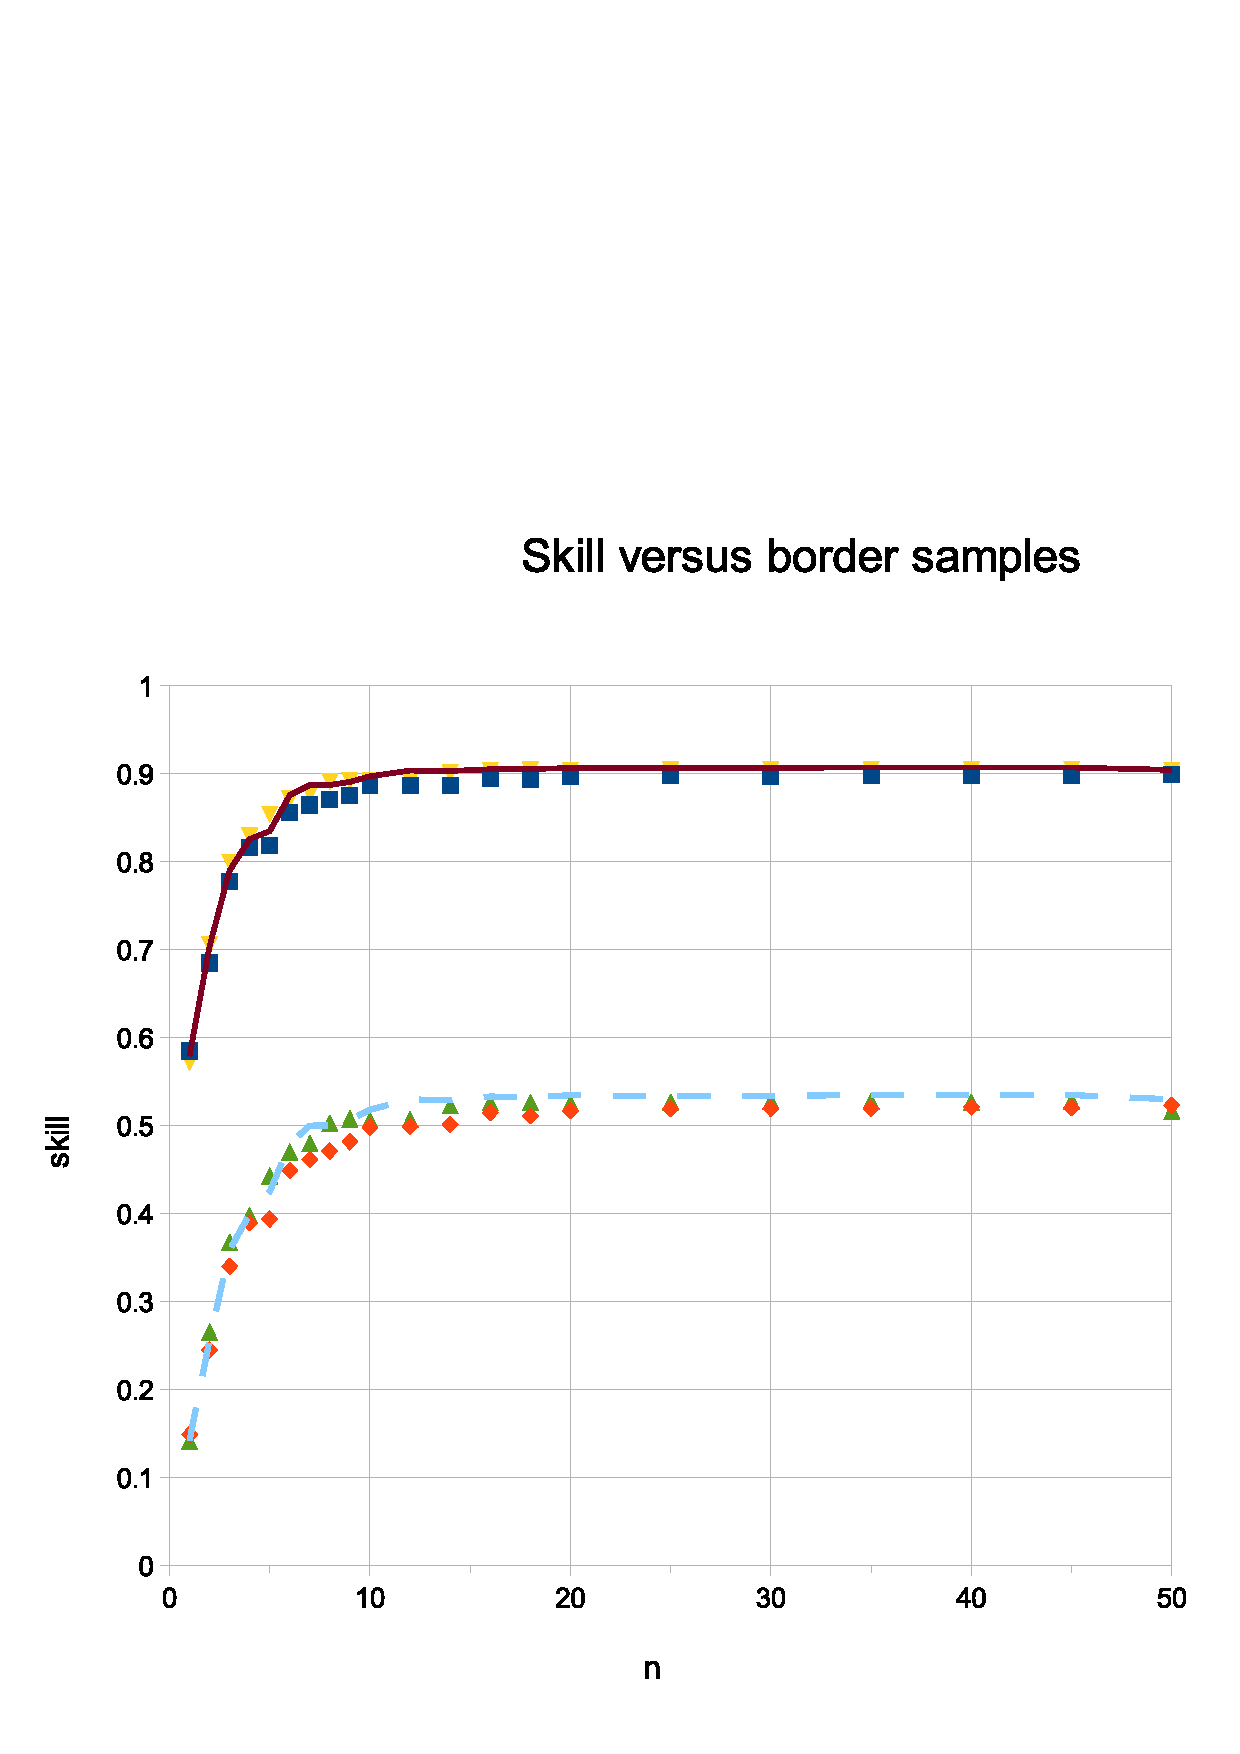
\includegraphics[width=0.9\textwidth]{skill_v_nb}
\caption{Classification accuracy and uncertainty coefficient for border-classification starting with probabilities from the class definitions, adaptive Gaussian filtering (AGF), and a support vector machine (SVM). Average of 20 trials.}
\label{skill_v_nb}
\end{figure}

The true border is also compared with those derived from AGF and LIBSVM
probability estimates in Figure \ref{border_vectors}.
The classes are again shown for reference.
While these borders contain several hundred samples for a clear view of where
they are located using each method, in fact the method works well with
surprisingly few samples.  Figure \ref{skill_v_nb} shows a plot of the skill
versus the number of border samples, where {\it U.C.} stands for
uncertainty coefficient. Note that the scores saturate at only about 20
samples meaning that for this problem at least, very fast classifications are
possible.

Unlike support vectors, the number of border samples required is approximately
independent of the number of training samples.
In addition to skill as a function of border samples for both AGF- and 
SVM-trained border-classifiers, Figure \ref{skill_v_nb} also shows results
for a border classifier trained from the mathematical definition of the 
classes themselves. 
The skill scores of this latter curve do not level any faster than the 
other two.
So long as the complexity of
the problem does not increase, adding new training samples does not increase
the number of border samples required for maximum accuracy.

\begin{figure}
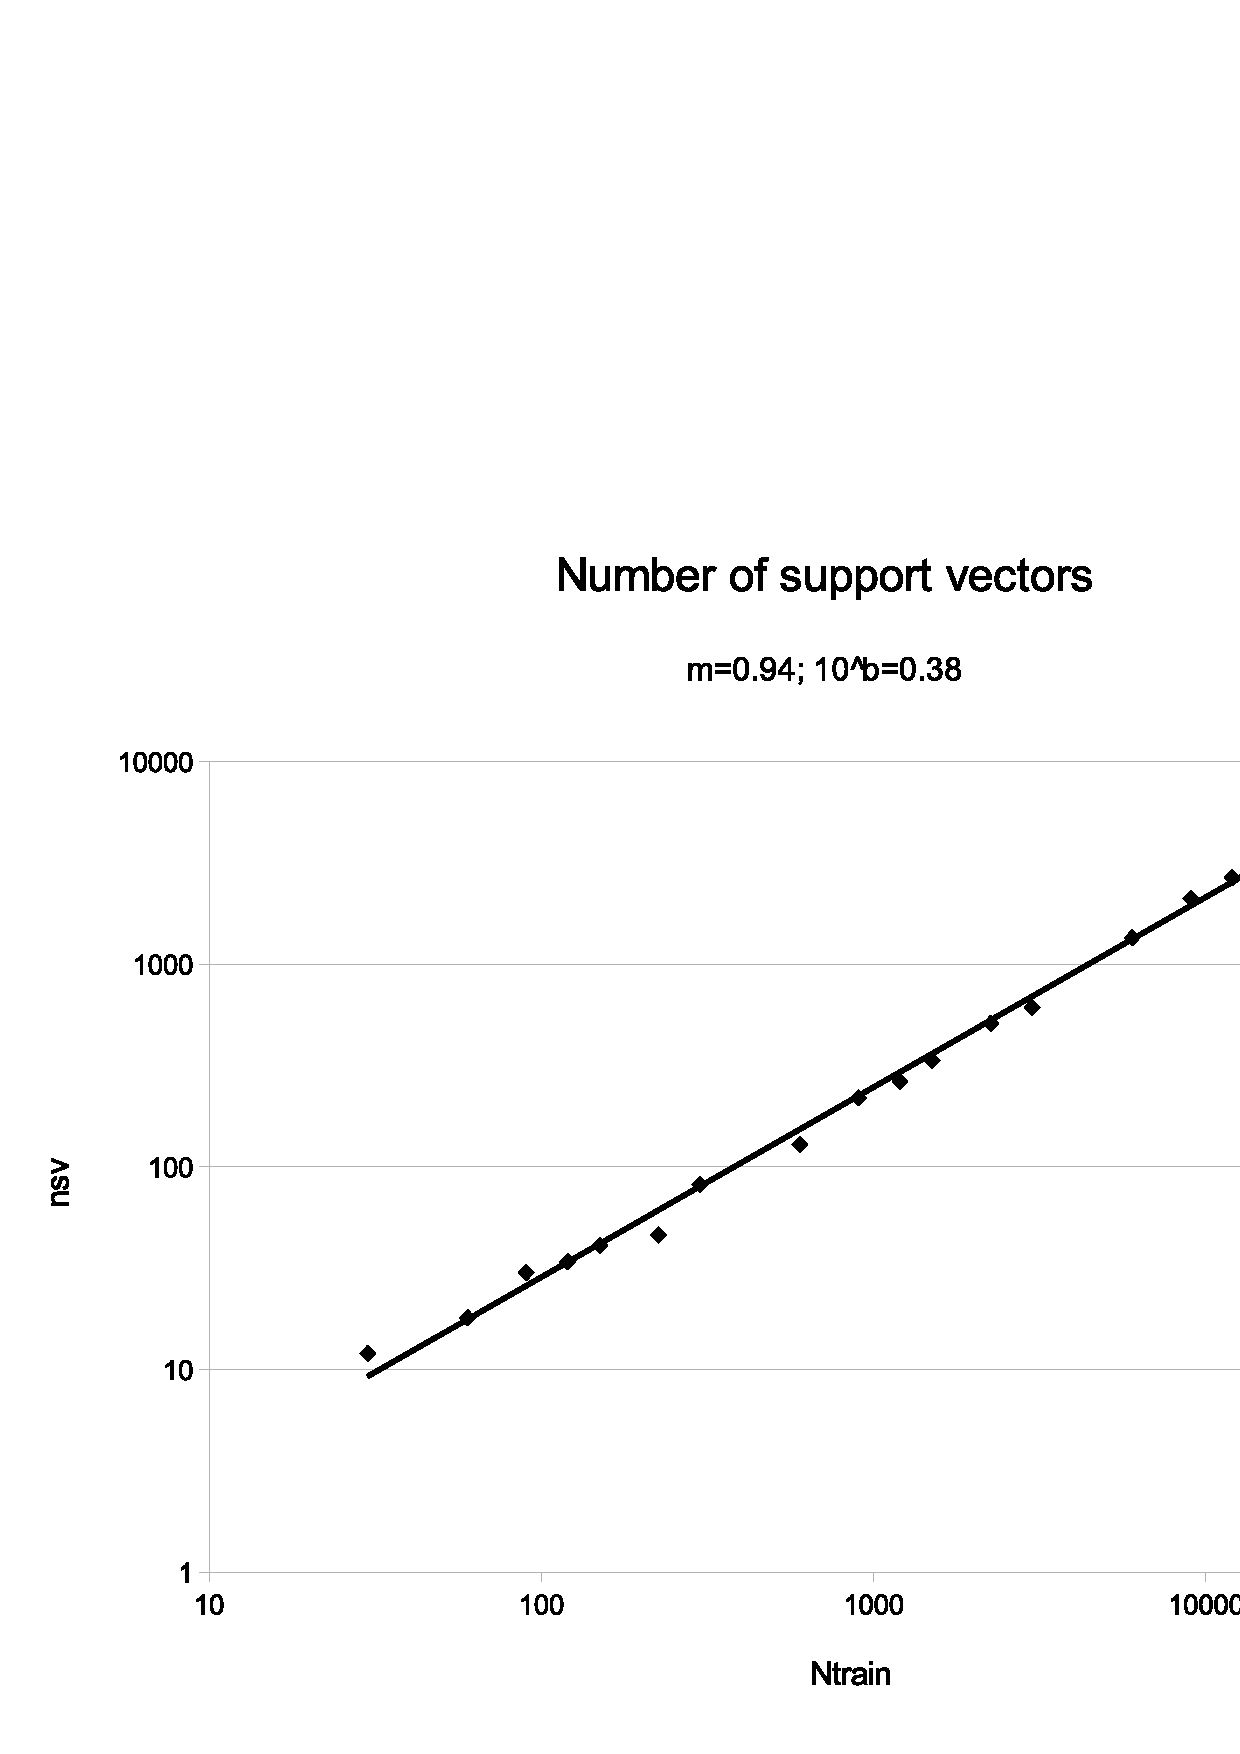
\includegraphics[width=0.9\textwidth]{nsv}
\caption{Number of support vectors against number of training vectors for pair of synthetic test classes. Fitted curve returns exponent of 0.94 and multiplication coefficient of 0.38.}
\label{nsv}
\end{figure}

Figure \ref{nsv} shows the number of support vectors as a versus the
number of training samples. The fitted curve is approximately linear 
with an exponent of 0.94 and multiplications coefficient of 0.38.
In other words, there will be approximately 38 \% as many support vectors as 
there are training vectors.

Of course it's possible to speed up an SVM by sub-sampling the training data
or the resulting support vectors.
In such case, the sampling must be done carefully so as not to reduce the
accuracy of the result.
Figure \ref{skill_v_nt} shows the effect on classification skill for the
synthetic test classes when the number of training samples is reduced.
Skill scores start to saturate at between 200 and 300 samples.
By contrast, figure \ref{skill_v_nb} suggests you need only 20 border samples
for good accuracy, so even with only 200 training samples you will still
have improved efficiency by using the borders technique.

\begin{figure}
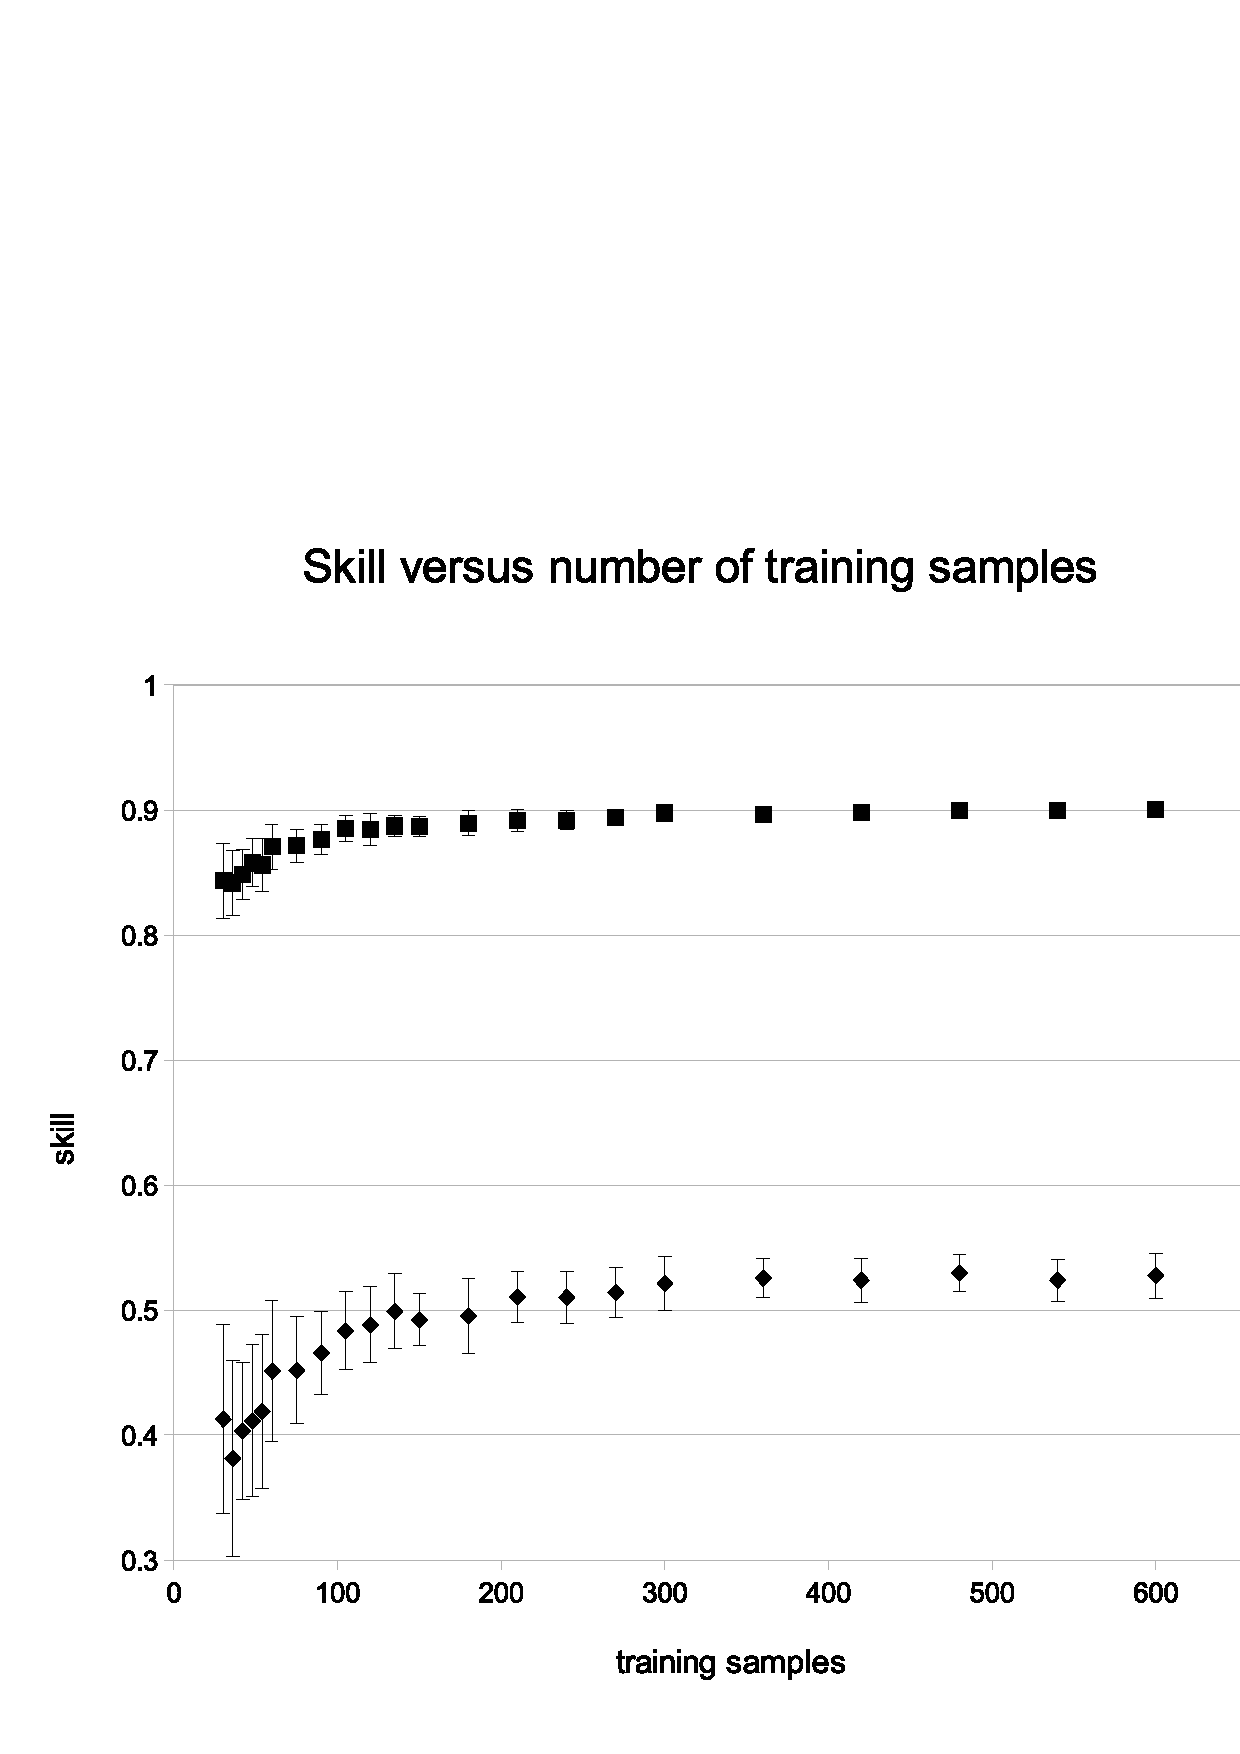
\includegraphics[width=0.9\textwidth]{skill_v_nt}
\caption{Classification accuracy and uncertainty coefficient for a support vector machine (SVM) trained with different numbers of samples.
Error bars represent the standard deviation of 20 trials.}
\label{skill_v_nt}
\end{figure}

This suggests a simple scaling law. The number of training samples required
for good accuracy, and hence the number of support vectors, 
should be proportional to the volume occupied by the
training data in the feature space: $n_0 \propto V$ where 
$n_0$ is the minimum number of training vectors and $V$ is volume.
Then the number of border vectors should be proportional to the volume
taken to the root of one less than the dimension of the feature space:
$n_{b0} \propto V^\frac{1}{D-1}$.
Putting it together, we can relate the two as follows:
\begin{equation}
	n_{b0} \propto n_0^\frac{1}{N-1}
\end{equation}
where $n_{b0}$ is the minimum number of border vectors required for good
accuracy.

\begin{figure}
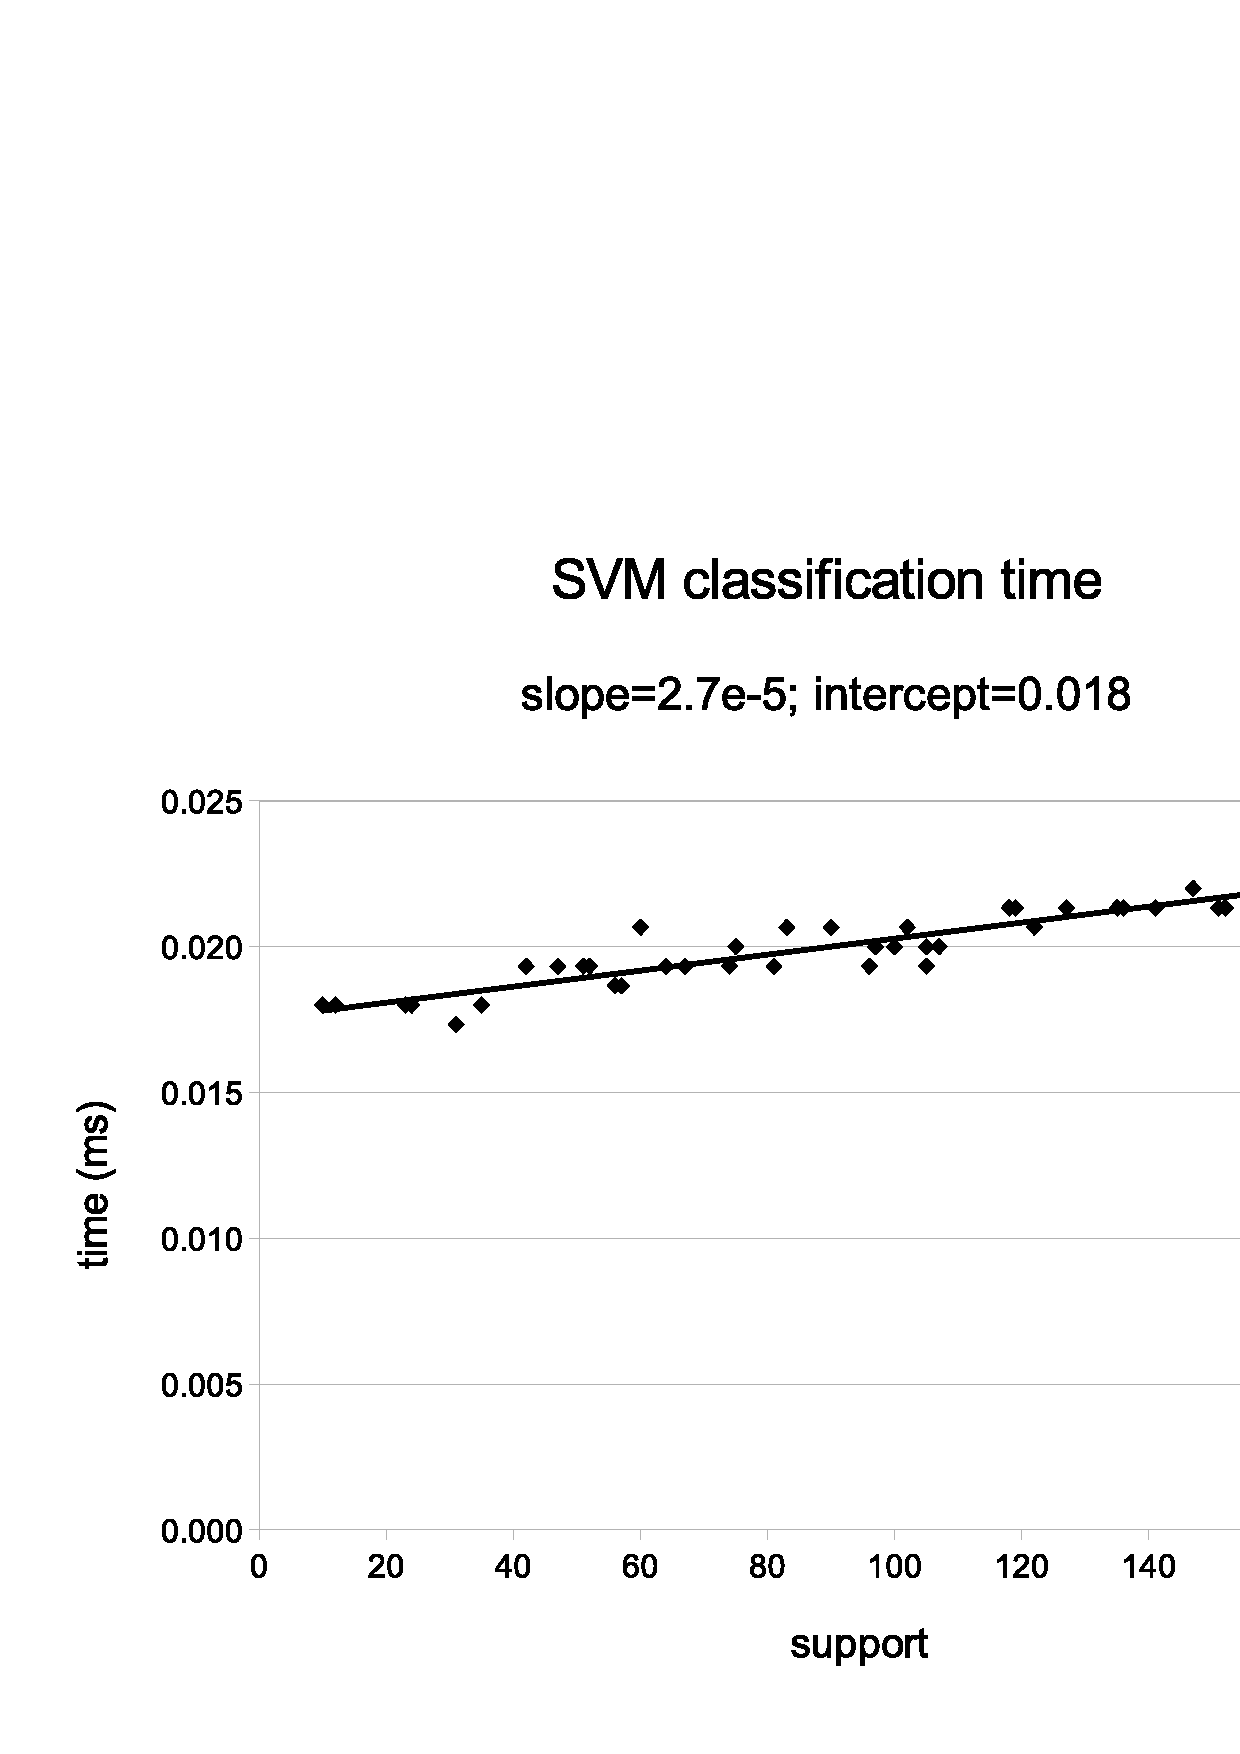
\includegraphics[width=0.9\textwidth]{svm_time}
\caption{Classification time for a SVM for a single test point as versus the number of support vectors.}
\label{svm_time}
\end{figure}

In other words, mapping only the border between classes should always be
faster than techniques that map the entirety of the class locations.
This includes kernel density methods including SVM as well
as similar methods such as learning vector quantization (LVQ) 
\citep{Kohonen2000, LVQ_PAK}
that attempt to create an ``idealized'' representation of the classes through
a set of ``codebook'' vectors.

\begin{figure}
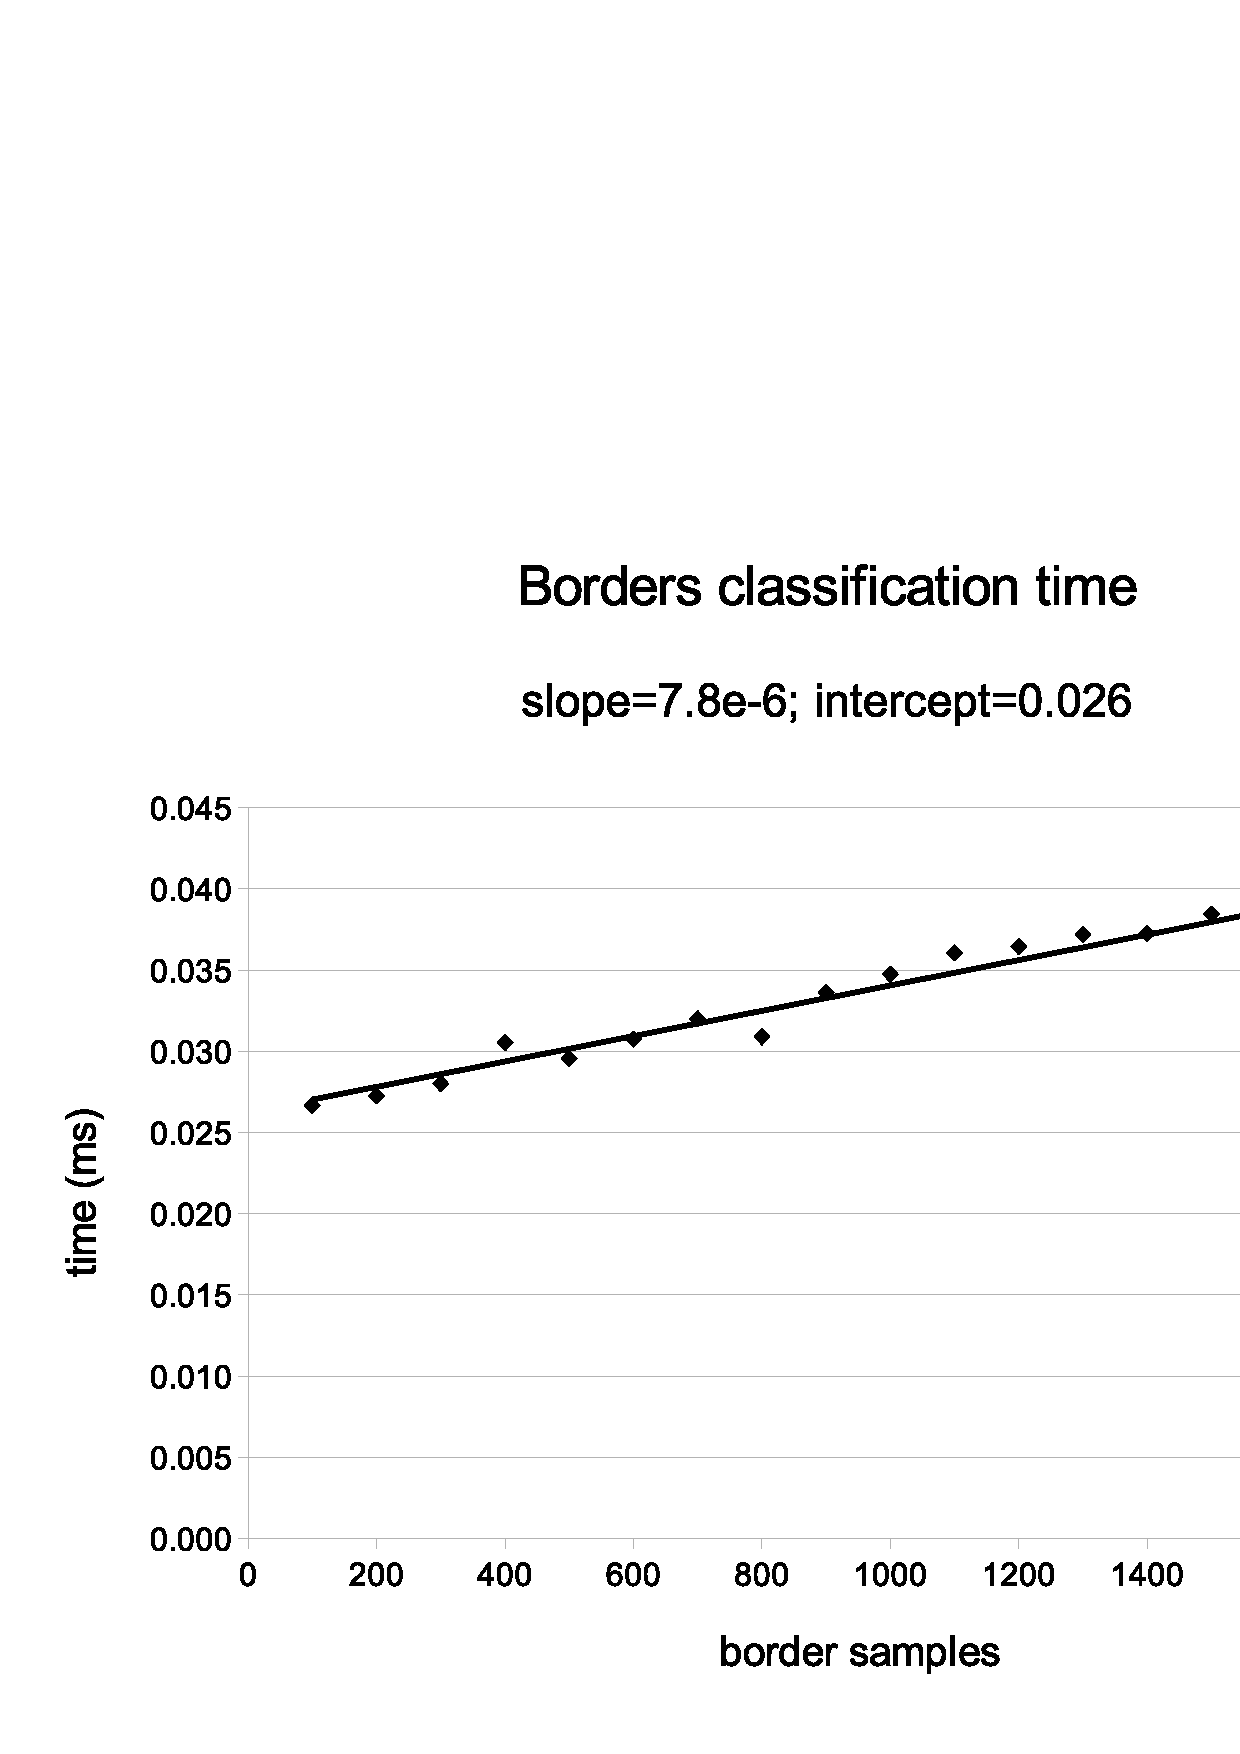
\includegraphics[width=0.9\textwidth]{border_time}
\caption{Classification time for a border classifier for a single test point versus the number of border samples.}
\label{border_time}
\end{figure}

To make this more concrete, Figure \ref{svm_time}
plots the classification time versus the number of support vectors
for a SVM
while Figure \ref{border_time} plots the classification time
versus the number of border samples for a border classifier.
Classification times are for a single test point.
Fitted straight lines are overlaid for each and the slope and intercept 
printed in the subtitle.

\begin{figure}
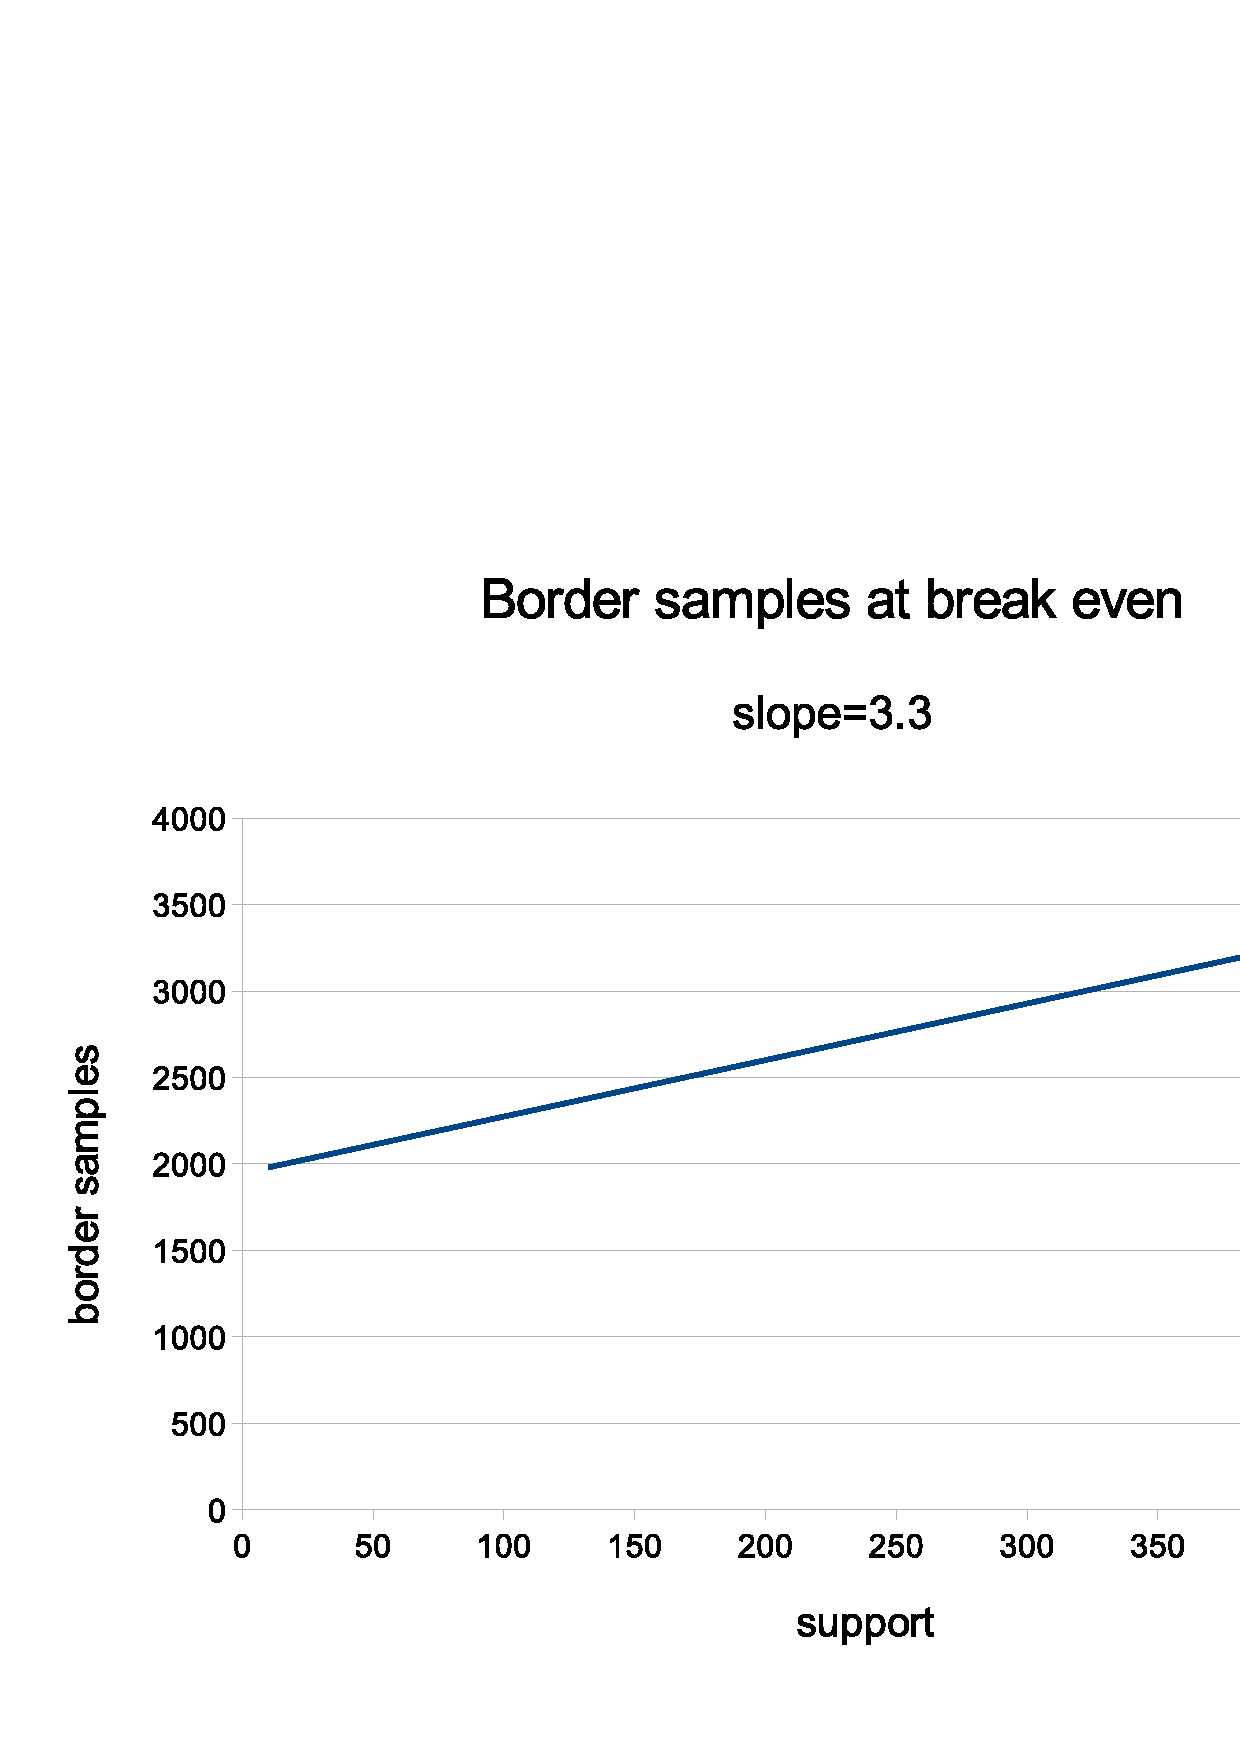
\includegraphics[width=0.9\textwidth]{break_even}
\caption{Number of border samples versus number of support vectors for equal classification times.}
\label{break_even}
\end{figure}

Figure \ref{break_even} plots the number of border vectors versus the number
of support vectors at the ``break even'' point: that is, the classfication
time is the same for each method.
This graph was simply derived from the fitted coefficents of the previous
two graphs.
It is misleadingly optimistic
since LIBSVM has a larger overhead than the border classifiers.
This overhead would be less significant for larger problems 
with the ``rule of thumb'' suggested by the slope 
that the number of border vectors should be less than three times the support
for a reasonable gain in efficiency.

Unfortunately the graph is not general: while the borders method scales linearly with
the number of classes, in LIBSVM there is some shared calculation for multi-class problems.
That is, some of the support vectors are shared between classes moreover the number will be different for each problem.
Model size comparisons between the two methods should ideally be between the total 
number of support vectors versus the total number of border vectors, not border (or support) vectors per class.
Both methods will tend to scale linearly with the number of attributes, with a small
component independent but a different amount for each method.
Once we take into account the number of classes and number of attributes, the
model for time complexity becomes quite complex so no attempt will be made here
to fit it since the comparison is only being tried on six different datasets.

\section{Case studies}

\begin{table}
		
\begin{tabular}{|l||ll|l|lll|l|ll|}
	\hline
Dataset	& Stat. & & KNN & AGF & & & Accel. & SVM & \\\hline
 & trials & $\datafraction$ & $k$ & $\kernelsum$ & $k$ & $\nborder$ & $\nborder$ & $\gamma$ & C\\\hline\hline
	heart & 10 & 0.4 & 11 & 10 & - & 100 & 100 & 0.01 & 0.5 \\
	shuttle & $10^*$ & 0.25 & 1 & 1.5 & 150 & 250 & 100 & 0.111 & 1 \\
	sat & $10^*$ & 0.31 & 5 & 5 & 100 & 200 & 200 & 0.1 & 50\\
	segment & 10 & 0.4 & 3 & 3 & 100 & 100 & 50 & 0.1 & 100 \\
	dna & $10^*$ & 0.372 & 11 & 20 & 300 & 500 & 1000 & 0.0055 & 1 \\
	splice & $10^*$ & 0.685 & 1 & 15 & - & 500 & 500 & 0.00167 & 1 \\
	codrna & $10^*$ & 0.82 & 11 & 10 & 200 & 500 & 500 & 0.125 & 1 \\
	letter & $10^*$ & 0.4 & 1 & 3 & 200 & 1000 & 75 & 0.065 & 1 \\
	pendigits & $10^*$ & 0.318 & 1 & 2 & 200 & 200 & 50 & 0.01 & 50 \\
	usps & $10^*$ & 0.216 & 1 & 1 & 100 & 250 & 50 & 0.004 & 1 \\
	mnist & 1 & 0.143 & 9 & 1 & 200 & 500 & 500 & 0.1 & 50 \\
	ijcnn1 & $10^*$ & 0.647 & 11 & 10 & 400 & 500 & 500 & 0.045 & 1 \\
	madelon & $10^*$ & 0.231 & 11 & 10 & 200 & 100 & 100 & 0.002 & 1 \\
	seismic & $10^*$ & 0.2 & 31 & 40 & 400 & 200 & 200 & 0.02 & 1 \\
	mushrooms & 10 & 0.4 & 3 & 3 & 300 & 500 & 200 & 0.0089 & 50 \\
	phishing & 10 & 0.4 & 3 & 7 & 250 & 500 & 500 & 0.00147 & 1 \\
	humidity & $10^*$ & 0.4 & 51 & 10 & 400 & 200 & 200 & 0.143 & 50 \\
	\hline
\end{tabular}


	\label{param}
	\caption{Summary of the parameters used in the numerical trials for each of the four methods: KNN ($k$-nearest-neighbours), AGF (adaptive Gaussian filtering), SVM (support vector machine) and ACC (``accelerated'' SVM).}
\end{table}

\begin{table}
	{\small
		\begin{table}
	\caption{Table of uncertainty coefficients for different multi-class
	configurations and solution methods.}
{\small
\begin{tabular}{|ll|llllll|}
\hline
 method & & letter & pendigits & sat & segment & shuttle & usps\\
\hline\hline
1 vs 1 & inv. & $0.938 \pm 0.004 $ & $0.984 \pm 0.002 $ & $0.804 \pm 0.008 $ & $0.924 \pm 0.01 $ & $0.954 \pm 0.003 $ & $0.93 \pm 0.005 $ \\
& iter. & $0.938 \pm 0.004 $ & $0.984 \pm 0.002 $ & $0.804 \pm 0.008 $ & $0.924 \pm 0.01 $ & $0.954 \pm 0.003 $ & $0.93 \pm 0.005 $ \\
hier. & rec. & $0.881 \pm 0.005 $ & $0.968 \pm 0.004 $ & $0.787 \pm 0.008 $ & $0.91 \pm 0.02 $ & $0.937 \pm 0.003 $ & $0.911 \pm 0.007 $ \\
 & iter. & $0.888 \pm 0.004 $ & $0.97 \pm 0.003 $ & $0.79 \pm 0.008 $ & $0.912 \pm 0.01 $ & $0.936 \pm 0.003 $ & $0.913 \pm 0.009 $ \\
emp. & rec. & $0.909 \pm 0.003 $ & $0.974 \pm 0.005 $ & $0.792 \pm 0.01 $ & $0.898 \pm 0.01 $ & $0.945 \pm 0.003 $ & $0.918 \pm 0.007 $ \\
 & iter & $0.913 \pm 0.002 $ & $0.975 \pm 0.005 $ & $0.795 \pm 0.009 $ & $0.909 \pm 0.01 $ & $0.945 \pm 0.003 $ & $0.921 \pm 0.006 $ \\
\hline
\end{tabular}
}
\end{table}

\begin{table}
	\caption{Table of Brier scores for different multi-class configurations. All probabilities included.}
{\small
\begin{tabular}{|ll|llllll|}
\hline
 method & & letter & pendigits & sat & segment & shuttle & usps\\
\hline\hline
1 vs 1 & inv. & $0.045 \pm 0.001 $ & $0.033 \pm 0.001 $ & $0.144 \pm 0.004 $ & $0.091 \pm 0.003 $ & $0.032 \pm 0.002 $ & $0.066 \pm 0.002 $ \\
 & iter. & $0.084 \pm 0.001 $ & $0.0392 \pm 0.001 $ & $0.146 \pm 0.004 $ & $0.094 \pm 0.003 $ & $0.033 \pm 0.001 $ & $0.068 \pm 0.002 $ \\
hier. & iter. & $0.0620 \pm 0.0009 $ & $0.042 \pm 0.002 $ & $0.151 \pm 0.004 $ & $0.096 \pm 0.005 $ & $0.042 \pm 0.001 $ & $0.073 \pm 0.003 $ \\
emp. & iter. & $0.0545 \pm 0.0009 $ & $0.039 \pm 0.003 $ & $0.149 \pm 0.004 $ & $0.098 \pm 0.004 $ & $0.038 \pm 0.001 $ & $0.070 \pm 0.002 $ \\
\hline
\end{tabular}
}
\end{table}

\begin{table}
	\caption{Table of Brier scores for different multi-class configurations. Winning classes only.}
{\small
\begin{tabular}{|ll|llllll|}
\hline
 method & & letter & pendigits & sat & segment & shuttle & usps\\
\hline\hline
1 vs 1 & inv. & $0.174 \pm 0.004 $ & $0.075 \pm 0.003 $ & $0.244 \pm 0.007 $ & $0.168 \pm 0.006 $ & $0.057 \pm 0.003 $ & $0.140 \pm 0.004 $ \\
 & iter. & $0.379 \pm 0.005 $ & $0.098 \pm 0.004 $ & $0.247 \pm 0.006 $ & $0.176 \pm 0.007 $ & $0.057 \pm 0.003 $ & $0.148 \pm 0.005 $ \\
hier. & rec. & $0.205 \pm 0.002 $ & $0.091 \pm 0.004 $ & $0.254 \pm 0.007 $ & $0.173 \pm 0.009 $ & $0.076 \pm 0.002 $ & $0.153 \pm 0.006 $ \\
 & iter. & $0.208 \pm 0.003 $ & $0.092 \pm 0.004 $ & $0.255 \pm 0.007 $ & $0.174 \pm 0.01 $ & $0.076 \pm 0.002 $ & $0.154 \pm 0.005 $ \\
emp. & rec. & $0.183 \pm 0.004 $ & $0.083 \pm 0.006 $ & $0.251 \pm 0.006 $ & $0.167 \pm 0.007 $ & $0.068 \pm 0.003 $ & $0.147 \pm 0.005 $ \\
 & iter. & $0.184 \pm 0.004 $ & $0.083 \pm 0.006 $ & $0.251 \pm 0.006 $ & $0.172 \pm 0.007 $ & $0.068 \pm 0.003 $ & $0.148 \pm 0.004 $ \\
\hline
\end{tabular}
}
\end{table}


	}
	\caption{Collation of results for numerical trials of the four different statistical classification methods over six different datasets.}
\end{table}

\begin{table}
	\begin{tabular}{|l|llllll|}
	\hline
& heart & shuttle & segment & sat & vehicle & humidity \\\hline
Features & 13 & 9 & 19 & 36 & 18 & 7 \\
Classes & 2 & 7 & 7 & 6 & 4 & 8 \\
	Train & 162 & 43500 & 1386 & 4435 & 846 & 86400 \\\hline
	Total support & $110\pm3$ & 1189 & $344\pm13$ & 1277 & & \\\hline
	Total borders & 100 & 2100 & 1050 & 2250 & & &\\\hline
\end{tabular}


	\caption{Total number of support vectors versus total number of border samples.}
\end{table}

Four classification models were tested on each of the six datasets described in
Section \ref{datasets}: k-nearest-neighbours (KNN), a borders model derived from
adaptive Gaussian filters (AGF), a support vector machine (SVM) and a borders
model derived from the previous SVM model (ACC for ``accelerated'' SVM).
KNN is useful to get a baseline accuracy from a stable, reliable method although
not always an efficient or high-performing one.
AGF-borders is compared with SVM-borders to see how much deriving the class borders
from a SVM improves accuracy over using a direct pointwise kernel density estimator.
The speed should be the same for the same number of border vectors.
Ideally, for large problems, the borders technique should produce significant time
savings over a SVM while having little effect on accuracy.

The parameters used for each method are summarized in Table \ref{param}.
Parameters for the AGF method were chosen strictly to maximize accuracy while
the single parameter, number of border samples, in the SVM-borders technique
was chosen for the best compromise between reduced accuracy and a speed
improvement over SVM. The parameter, $k$, for AGF is the number of nearest
neighbours used when computing the probabilities: 
while the order of the method, $O(n)$, remains the same, nonetheless it can produce a significant speed improvement for large problems.
The parameter, $n_{samp}$, is the number of class borders used in both 
AGF and SVM-borders.

For SVM, a Gaussian kernel is used:
\begin{equation}
	K(\vec x, \vec y) = \exp \left ( -\gamma | \vec x - \vec y |^2 \right )
\end{equation}
where $\gamma$ is a tunable parameter. 
$C$ is a cost parameter added to reduce over-fitting.
For more information, see \citet{Chang_Lin2011} and \citet{kernel_intro}.

\bibliography{../agf_bib}

\end{document}
